% !TEX root = paper.tex
% !TEX encoding = UTF-8 Unicode



% !TEX root = paper.tex
% !TEX encoding = UTF-8 Unicode

\begin{figure}
\begin{subfigure}[b]{\linewidth}
\begin{center}
\caption{Russian-English}
\label{fig:mean_adequacy_gain_ru}
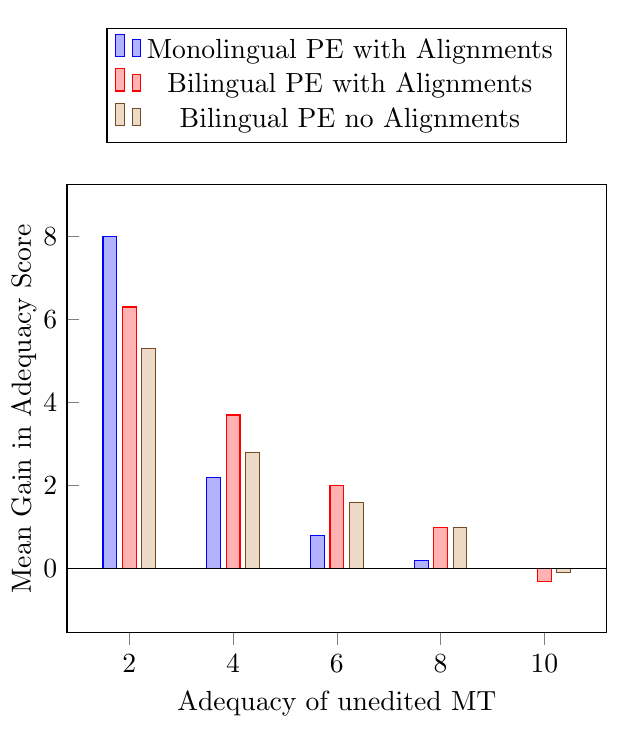
\begin{tikzpicture}[trim left={(-0.5,0)},trim axis right]
\begin{axis}[
	x tick label style={
		/pgf/number format/1000 sep=},
	ylabel shift={-0.15cm},
	ylabel=Mean Gain in Adequacy Score,
	xlabel={Adequacy of unedited MT},
%	ymin={0.1},
	enlargelimits=0.15,
	legend style={at={(0.5,1.35)},anchor=north},
	ybar,
	bar width=5pt,
	xtick pos=left,
	ytick pos=left,
%	ymin=0.0,
]
\addplot 
	coordinates {(2,8.0) (4,2.2)
		 (6,0.8) (8,0.2) (10,0)};

\addplot 
	coordinates {(2,6.3) (4,3.7)
		 (6,2.0) (8,1.0) (10,-0.3)};

\addplot 
	coordinates {(2,5.3) (4,2.8)
		 (6,1.6) (8,1.0) (10,-0.1)};

\addplot[black,sharp plot,update limits=false] 
	coordinates {(-1,0) (12,0)};

\legend{Monolingual PE with Alignments,Bilingual PE with Alignments,Bilingual PE no Alignments}
\end{axis}
\end{tikzpicture}
\end{center}
\end{subfigure}
\ \\ \ \\
\begin{subfigure}[b]{\linewidth}
\begin{center}
\caption{Spanish-English}
\label{fig:mean_adequacy_gain_es}
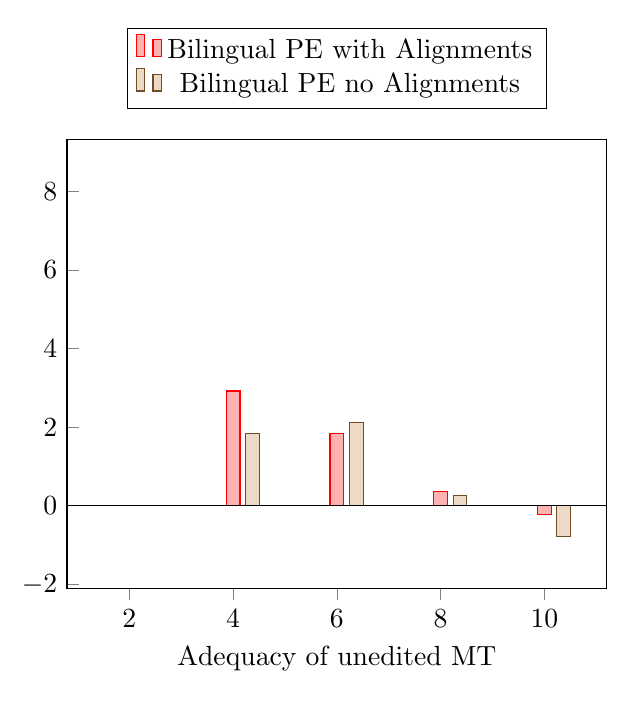
\begin{tikzpicture}[trim left={(-0.5,0)},trim axis right]
\begin{axis}[
	x tick label style={
		/pgf/number format/1000 sep=},
	ylabel shift={-0.15cm},
%	ylabel=Mean Gain in Adequacy Score,
	xlabel={Adequacy of unedited MT},
%	ymin={0.1},
	enlargelimits=0.15,
	legend style={at={(0.5,1.25)},anchor=north},
	ybar,
	bar width=5pt,
	xtick pos=left,
	xmin=2,
	ytick pos=left,
	ymax = 8,
%	ymin=0.0,
]
\addplot 
	coordinates {};

%	Gain with align	Gain w/o align
%2		
%4	2.92	1.84
%6	1.85	2.11
%8	0.36	0.25
%10	-0.22	-0.78

\addplot coordinates {(4,2.92) (6,1.85) (8,0.36) (10,-0.22) };
\addplot coordinates {(4,1.84) (6,2.11) (8,0.25) (10,-0.78) };

%\addplot coordinates {(4,2.6) (6,1.7272727272727273) (8,0.8181818181818182) (10,-0.07692307692307693) };
%\addplot coordinates {(4,2.0) (6,2.090909090909091) (8,0.9090909090909091) (10,-0.6153846153846154) };

\addplot[black,sharp plot,update limits=false] 
	coordinates {(-1,0) (12,0)};

\legend{Bilingual PE with Alignments,Bilingual PE no Alignments}
\end{axis}
\end{tikzpicture}
\end{center}
\end{subfigure}
\caption{Mean gain in adequacy score over unedited MT, categorized by the adequacy score of the unedited MT.}
\label{fig:mean_adequacy_gain}
\end{figure}





\subsection{Rating Adequacy of Russian-English}

%\subsection{Rating of translations}

An experienced English-Russian translator and grader rated all post-edited segments as well as the MT segments.%
%in both human-readable tabular form and machine-readable CSV form in the attached dataset supplement.}
%
The rater was presented with blocks of 10 lines arranged in a vertical list:
%
the first line was a source segment, 
%
the second was its reference translation, and 
%
below these were eight translations for the segment 
%
(the MT, one monolingual post-edited translation from \citet{2014_WMT_Schwartz_etal}, and six bilingual post-edited translations) 
%
listed in random order. 
%
The rater was asked to classify all the segment translations on an adequacy scale (see Table \Vref{judge_guidelines_russian}) ranging from 2 (translation makes no sense) to 12 (translation is superior to the reference translation). 


\subsection{Rating Adequacy of Russian-English}

One experienced Spanish-English translator and grader and one Spanish-English bilingual rated all post-edited segments as well as the MT segments.
%
They did this in cooperation.
%
The raters were presented with blocks of six lines arranged in a vertical list: the first line was a source segment, the second was its machine translation, and below these were four translations for the segment listed in random order.
%
The raters were asked to classify all the segment translations on an adequacy scale (see Table \Vref{judge_guidelines_spanish}) ranging from 2 (translation makes no sense) to 10 (the meaning of the Spanish sentence is fully conveyed in the English translation). 
% 
For the rating of the segments in this experiment the top category used for the evaluation of the Russian segments was removed because in the Spanish experiment we did not use a reference translation.

\section{Results}
\label{sec:results}

\subsection{Russian-English Adequacy}

%The post-edited English segments

The mean adequacy score when bilingual participants were presented with alignments was 8.35.
%
When alignments were omitted from the post-editing tool, the mean adequacy score was 7.85.  
%
A Wilcoxon signed-rank test \citep{1945_Wilcoxon} showed that when participants were presented with alignments the ratings of their translations were significantly higher than when participants post-edited without access to alignments (N = 6, Z = -2.207, p = 0.027).


% !TEX root = paper.tex
% !TEX encoding = UTF-8 Unicode

\begin{figure*}[t]
\begin{subfigure}[b]{.5\linewidth}
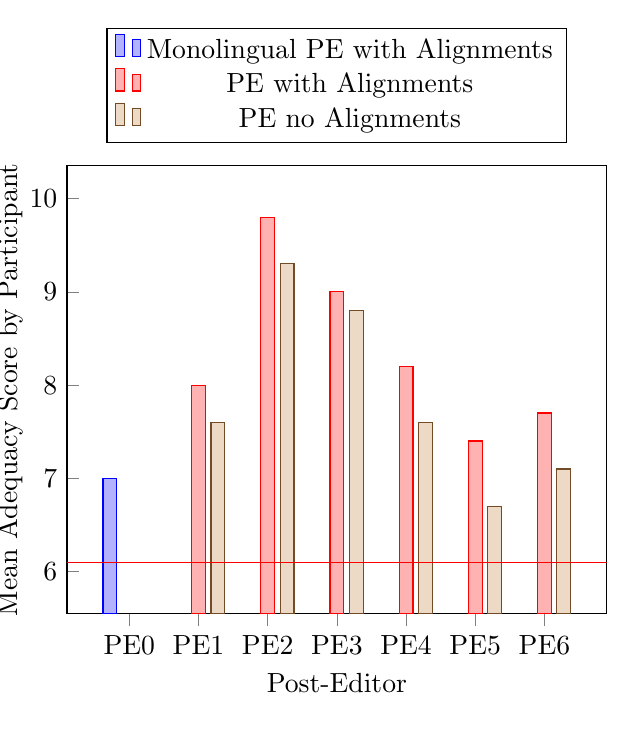
\begin{tikzpicture}[trim left={(-0.5,0)},trim axis right]
\begin{axis}[
    ybar,
    enlargelimits=0.15,
    legend style={at={(0.5,1.05)},anchor=south},
   ylabel={Mean Adequacy Score by Participant},
   xlabel={Post-Editor},
   % symbolic x coords={PE0,PE1,PE2,PE3,PE4,PE5,PE6},
    xtick={0,1,2,3,4,5,6},
    xticklabels={PE0,PE1,PE2,PE3,PE4,PE5,PE6},
	xtick pos=left,
	ytick pos=left,
	ylabel shift={-0.15cm},
    %xtick=data,
    %nodes near coords,
    %nodes near coords align={vertical},
    bar width=5pt
    ]

\addplot coordinates { (0,7.0) (0,6.1)};
\addplot coordinates { (1,8.0) (2,9.8) (3,9.0) (4,8.2) (5,7.4) (6,7.7)};
\addplot coordinates { (1,7.6) (2,9.3) (3,8.8) (4,7.6) (5,6.7) (6,7.1)};

\addplot[red,sharp plot,update limits=false] 
	coordinates {(-1,6.1) (8,6.1)};
	%node[above] at (axis cs:3,6.1) {Unedited MT};
	
%%\addplot coordinates {(tool8,1) (tool9,1) (tool10,1)};
\legend{Monolingual PE with Alignments, PE with Alignments,PE no Alignments}
\end{axis}
\end{tikzpicture}
\caption{Russian-English}
\label{fig:mean_adequacy_score_per_posteditor_ru}
\end{subfigure}
\begin{subfigure}[b]{.5\linewidth}
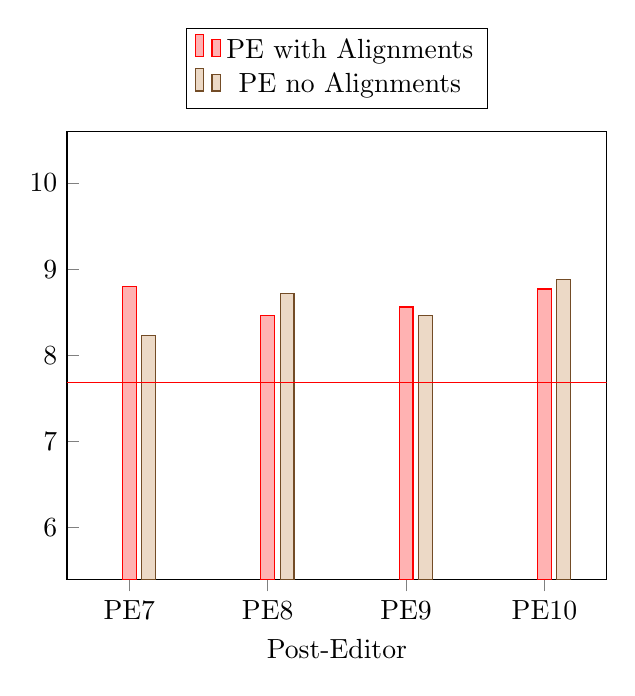
\begin{tikzpicture}[trim left={(-0.5,0)},trim axis right]
\begin{axis}[
    ybar,
    enlargelimits=0.15,
    legend style={at={(0.5,1.05)},anchor=south},
%   ylabel={Mean Adequacy Score by Participant},
   xlabel={Post-Editor},
   % symbolic x coords={PE0,PE1,PE2,PE3,PE4,PE5,PE6},
    xtick={1,2,3,4},
    xticklabels={PE7,PE8,PE9,PE10},
	xtick pos=left,
	ytick pos=left,
	ylabel shift={-0.15cm},
	ymin=6,
	ymax=10,
    %xtick=data,
    %nodes near coords,
    %nodes near coords align={vertical},
    bar width=5pt
    ]

\addplot coordinates {};
\addplot coordinates {(1,8.8) (2,8.461538461538462) (3,8.56) (4,8.76923076923077) };
\addplot coordinates {(1,8.23076923076923) (2,8.72) (3,8.461538461538462) (4,8.88) };
\addplot[red,sharp plot,update limits=false] coordinates { (-1,7.686274509803922) (12,7.686274509803922) };

%%\addplot coordinates {(tool8,1) (tool9,1) (tool10,1)};
\legend{PE with Alignments,PE no Alignments}
\end{axis}
\end{tikzpicture}
\caption{Spanish-English}
\label{fig:mean_adequacy_score_per_posteditor_es}
\end{subfigure}
\caption{Mean adequacy score per post-editor. The red horizontal line indicates the mean adequacy score (Russian-English: 6.1; Spanish-English: 7.7) of the unedited MT.}
\label{fig:mean_adequacy_score_per_posteditor}
\end{figure*}


\subsection{Spanish-English Adequacy}

The mean adequacy score when Spanish bilingual participants were presented with alignments was 8.65. When alignments were omitted from the post-editing tool, the mean adequacy score was 8.57. These means were not significantly different.

\subsection{Analysis}

This finding indicates that, at least for this language pair and data set, bilingual post-editors produce higher quality translations when presented with bilingual alignment links between source words and machine-translated target words.

In addition to rating each post-edited translation, our bilingual human judge rated the adequacy of the unedited MT segments.
%
We thereby obtained direct human judgements of MT quality.%
%
Because we care about the adequacy of post-edited translations, we consider actual human judgements to be preferable to automated metrics such as BLEU \citep{2002_ACL_Papineni_etal}, which at best serve as a flawed proxy for human judgements.

We partition the data according to the MT quality as measured by our human judge in terms of adequacy.
%
For each partition, we then calculate the mean adequacy score of post-edited segments, once for the case where post-editors were presented with alignment data, and once for the case where alignments were not presented.
%
In addition, we perform the same average calculation for the monolingual post-edited segments of Docs A and B from \citet{2014_WMT_Schwartz_etal}.
%
The results are shown in Figure \ref{fig:mean_adequacy_score}.


%\clearpage 



% !TEX root = paper.tex
% !TEX encoding = UTF-8 Unicode

\begin{figure}
\begin{subfigure}[b]{\linewidth}
\begin{center}
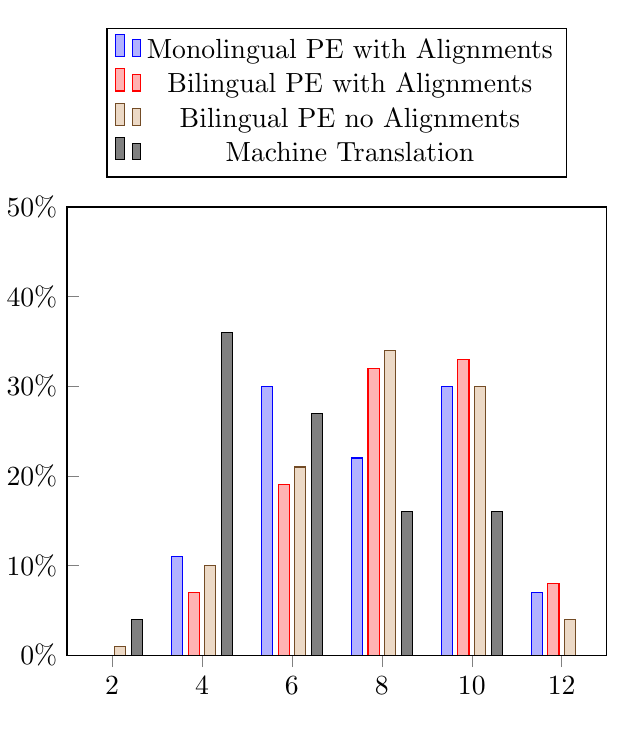
\begin{tikzpicture}[trim left={(-0.5,0)}]
\begin{axis}[
	%at={(10,0)},
	ymin=0,
	x tick label style={
		/pgf/number format/1000 sep=},
	ylabel shift={-0.15cm},
	ytick={0,10,20,30,40,50},
	yticklabels={0\%,10\%,20\%,30\%,40\%,50\%},
%	ymin={0},
	ymax={50},
%	ylabel={\%},
%	enlargelimits=0.15,
	xtick pos=left,
	ytick pos=left,
%	xlabel={XXXX YYY ZZZZ},
	%,
%	legend style={at={(0.5,-0.15)}},
%		anchor=north,legend columns=-1},
	legend style={at={(0.5,1.40)},anchor=north},
	ybar,
	bar width=4pt,
]
\addplot 
	coordinates {(4,11) (6,30) (8,22) (10,30) (12,7)};

\addplot 
	coordinates {(4,7) (6,19) (8,32) (10,33) (12,8)};

\addplot 
	coordinates {(2,1) (4,10) (6,21) (8,34) (10,30) (12,4)};

\addplot 
	coordinates {(2,4) (4,36) (6,27) (8,16) (10,16)};

\addplot[black,sharp plot,update limits=false] 
	coordinates {(-1,0) (14,0)};
	
\legend{Monolingual PE with Alignments,Bilingual PE with Alignments,Bilingual PE no Alignments, Machine Translation}
\end{axis}
\end{tikzpicture}
\end{center}
\caption{Russian-English}
\label{fig:percentage_segments_ru}
\end{subfigure}
\ \\
\begin{subfigure}[b]{\linewidth}
\begin{center}
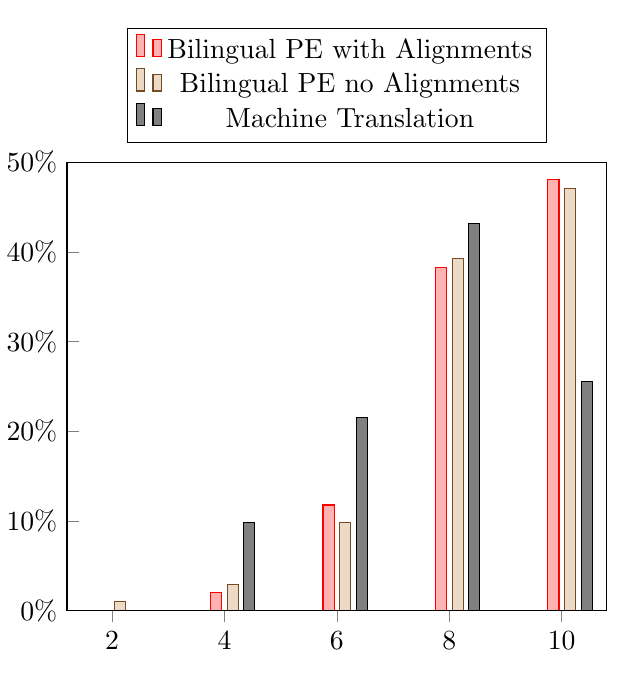
\begin{tikzpicture}[trim left={(-0.5,0)}]
\begin{axis}[
	%at={(10,0)},
	ymin=0,
	x tick label style={
		/pgf/number format/1000 sep=},
	ylabel shift={-0.15cm},
	ytick={0,10,20,30,40,50},
	yticklabels={0\%,10\%,20\%,30\%,40\%,50\%},
%	ymin={0},
	ymax={50},
%	ylabel={\%},
%	enlargelimits=0.15,
	xtick pos=left,
	ytick pos=left,
%	xlabel={XXXX YYY ZZZZ},
	%,
%	legend style={at={(0.5,-0.15)}},
%		anchor=north,legend columns=-1},
	legend style={at={(0.5,1.30)},anchor=north},
	ybar,
	bar width=4pt,
]
\addplot 
	coordinates {};

\addplot coordinates {(4,1.9607843137254901) (6,11.76470588235294) (8,38.23529411764706) (10,48.03921568627451) };
\addplot coordinates {(2,0.9803921568627451) (4,2.941176470588235) (6,9.803921568627452) (8,39.21568627450981) (10,47.05882352941176) };
\addplot coordinates {(4,9.803921568627452) (6,21.568627450980394) (8,43.13725490196079) (10,25.49019607843137) };

\addplot[black,sharp plot,update limits=false] 
	coordinates {(-1,0) (14,0)};
	
\legend{Bilingual PE with Alignments,Bilingual PE no Alignments, Machine Translation}
\end{axis}
\end{tikzpicture}
\end{center}
\caption{Spanish-English}
\label{fig:percentage_segments_es}
\end{subfigure}
\caption{Percentage of segments judged to be in each adequacy category. For each language pair, we report percentages for raw (unedited) machine translation output, as well as output post-edited by a bilingual post-editor with access to alignments and without access to alignments. For Russian-English, we additionally report percentages for output post-edited by a monolingual post-editor \citep{2014_WMT_Schwartz_etal} with access to alignments.}
\label{fig:percentage_segments}
\end{figure}



We observe that when MT quality was poor (adequacy categories 2--6), bilingual post-editors consistently produced higher quality post-edited translations when alignments were shown.
%
When MT quality was high (adequacy categories 8--10), little or no impact to adequacy quality was observed when alignments were shown. 
%
By subtracting the adequacy score of each machine translated segment, we obtain the adequacy gain obtained by post-editing.
%
The above effect can be seen clearly in Figure \Vref{fig:mean_adequacy_gain}, where we show mean gain in adequacy over unedited MT;
%
post-editing makes the most difference when MT quality is poor, and in those cases the presence of alignment links improves post-editing as measured by adequacy.


In Figure \ref{fig:mean_adequacy_score_per_posteditor}, we examine the effect that alignment link visualization has on each bilingual post-editor.
%
We observe that post-editing quality varies widely between post-editors (with PE2 and PE3 performing best).
%
For all six bilingual post-editors, we observe higher mean adequacy scores when alignment links were presented than when they were omitted from the post-editing tool.
%
We also note that when alignment links were absent, one bilingual post-editor (PE5) performed worse than the monolingual post-editor (PE0) from \citet{2014_WMT_Schwartz_etal}.
%
When compared to the unedited machine translations, post-editing resulted in improved mean adequacy for all post-editors, both bilingual and monolingual.

Finally, in Figure \ref{fig:percentage_segments} we present histograms graphing the percentage of segments in each adequacy category.
%
We observe that the majority of unedited machine translations are of relatively poor quality, falling mostly into categories 4 and 6. %, and a few scoring as 12.
%
%The monolingual post-editor from \citet{2014_WMT_Schwartz_etal} was able to skew the quality histogram somewhat to the right, with most segments scored as 6 or 10, and a few scored as better than the reference (12).
The monolingual post-editor improved MT quality somewhat, with most segments scoring as 6 or 10.
%
The histogram for bilingual post-editors using no alignments skewed further to the right, peaking at 8.
%
The histogram for bilingual post-editors with access to alignments skews farthest to the right, peaking at 10.



